\begin{recipe}{Italian Chicken \& Pepper Sandwiches}{4 Portions}{35 Minutes}

\ingredient[24]{Oz}{Yukon Gold Potatoes}
\ingredient[]{}{Olive Oil}
\ingredient[]{}{Salt}
\ingredient[]{}{Pepper}
Cut potatoes into \fr{1}{2}-inch-thick wedges. Toss on a baking sheet with a large drizzle (or spray) of oil, salt, and pepper. Roast on top rack until golden brown and crispy, 20--25 minutes.\\

\newstep
\ingredient[2]{}{Yellow Onions}
\ingredient[2]{}{Long Green Peppers}
\ingredient[]{}{Olive Oil}
Halve, peel, and thinly slice onions. Halve, core, and thinly slice green peppers into strips. Heat a large drizzle of oil in a large pan over medium-high heat. Add onions and green peppers. Cook, stirring occasionally, until softened and lightly browned, 5--7 minutes. Season with salt and pepper. Turn off heat, and transfer to plate.\\

\newstep
\ingredient[20]{Oz}{Chicken Breast Strips}
\ingredient[]{}{Salt}
\ingredient[]{}{Pepper}
\ingredient[]{}{Olive Oil}
\ingredient[2]{Tbsp}{Italian Seasoning}
\ingredient[2]{???}{Chicken Stock Concentrate}
\ingredient[4]{Tbsp}{Water}
Pat chicken dry with paper towels. Season generously with salt and pepper. Heat a large drizzle of olive oil in pan used for veggies over medium-high heat. Add chicken in a single layer, and season with Italian Seasoning. Cook, stirring occasionally, until chicken is browned and cooked through, 4--6 minutes. Stir in stock concentrate and 4 Tbsp water. Season with salt and pepper. Return cooked veggies to pan, and stir to combine. Turn off heat.\\

\newstep
\ingredient[4]{}{Demi-Baguettes}
\ingredient[1]{Tsp}{Garlic Powder}
\ingredient[]{}{Olive Oil}
Slice baguettes lengthwise, stopping before you get all the way through. Sprinkle garlic powder onto the cut sides, and drizzle (or spray) with olive oil. Place, cut sides up, on a second baking sheet. Toast on middle rack until golden, 2--3 minutes.\\

\newstep
\ingredient[4]{Tbsp}{Mayonnaise}
\ingredient[4]{Tbsp}{Sour Cream}
\ingredient[1]{Tsp}{Garlic Powder}
\ingredient[]{}{Salt}
\ingredient[]{}{Pepper}
In a small bowl, combine mayonnaise, sour cream, and garlic powder. Season with salt and pepper.\\

\newstep
\ingredient[\fr{1}{2}]{Cup}{Mozzarella Cheese}
Spread bottom halves of toasted garlic buns with half the garlic sauce. Top the chicken and veggie mixture, then sprinkle with mozzarella. Return to middle rack until cheese melts, 2--3 minutes.

\end{recipe}

\begin{center}
~\\~\\
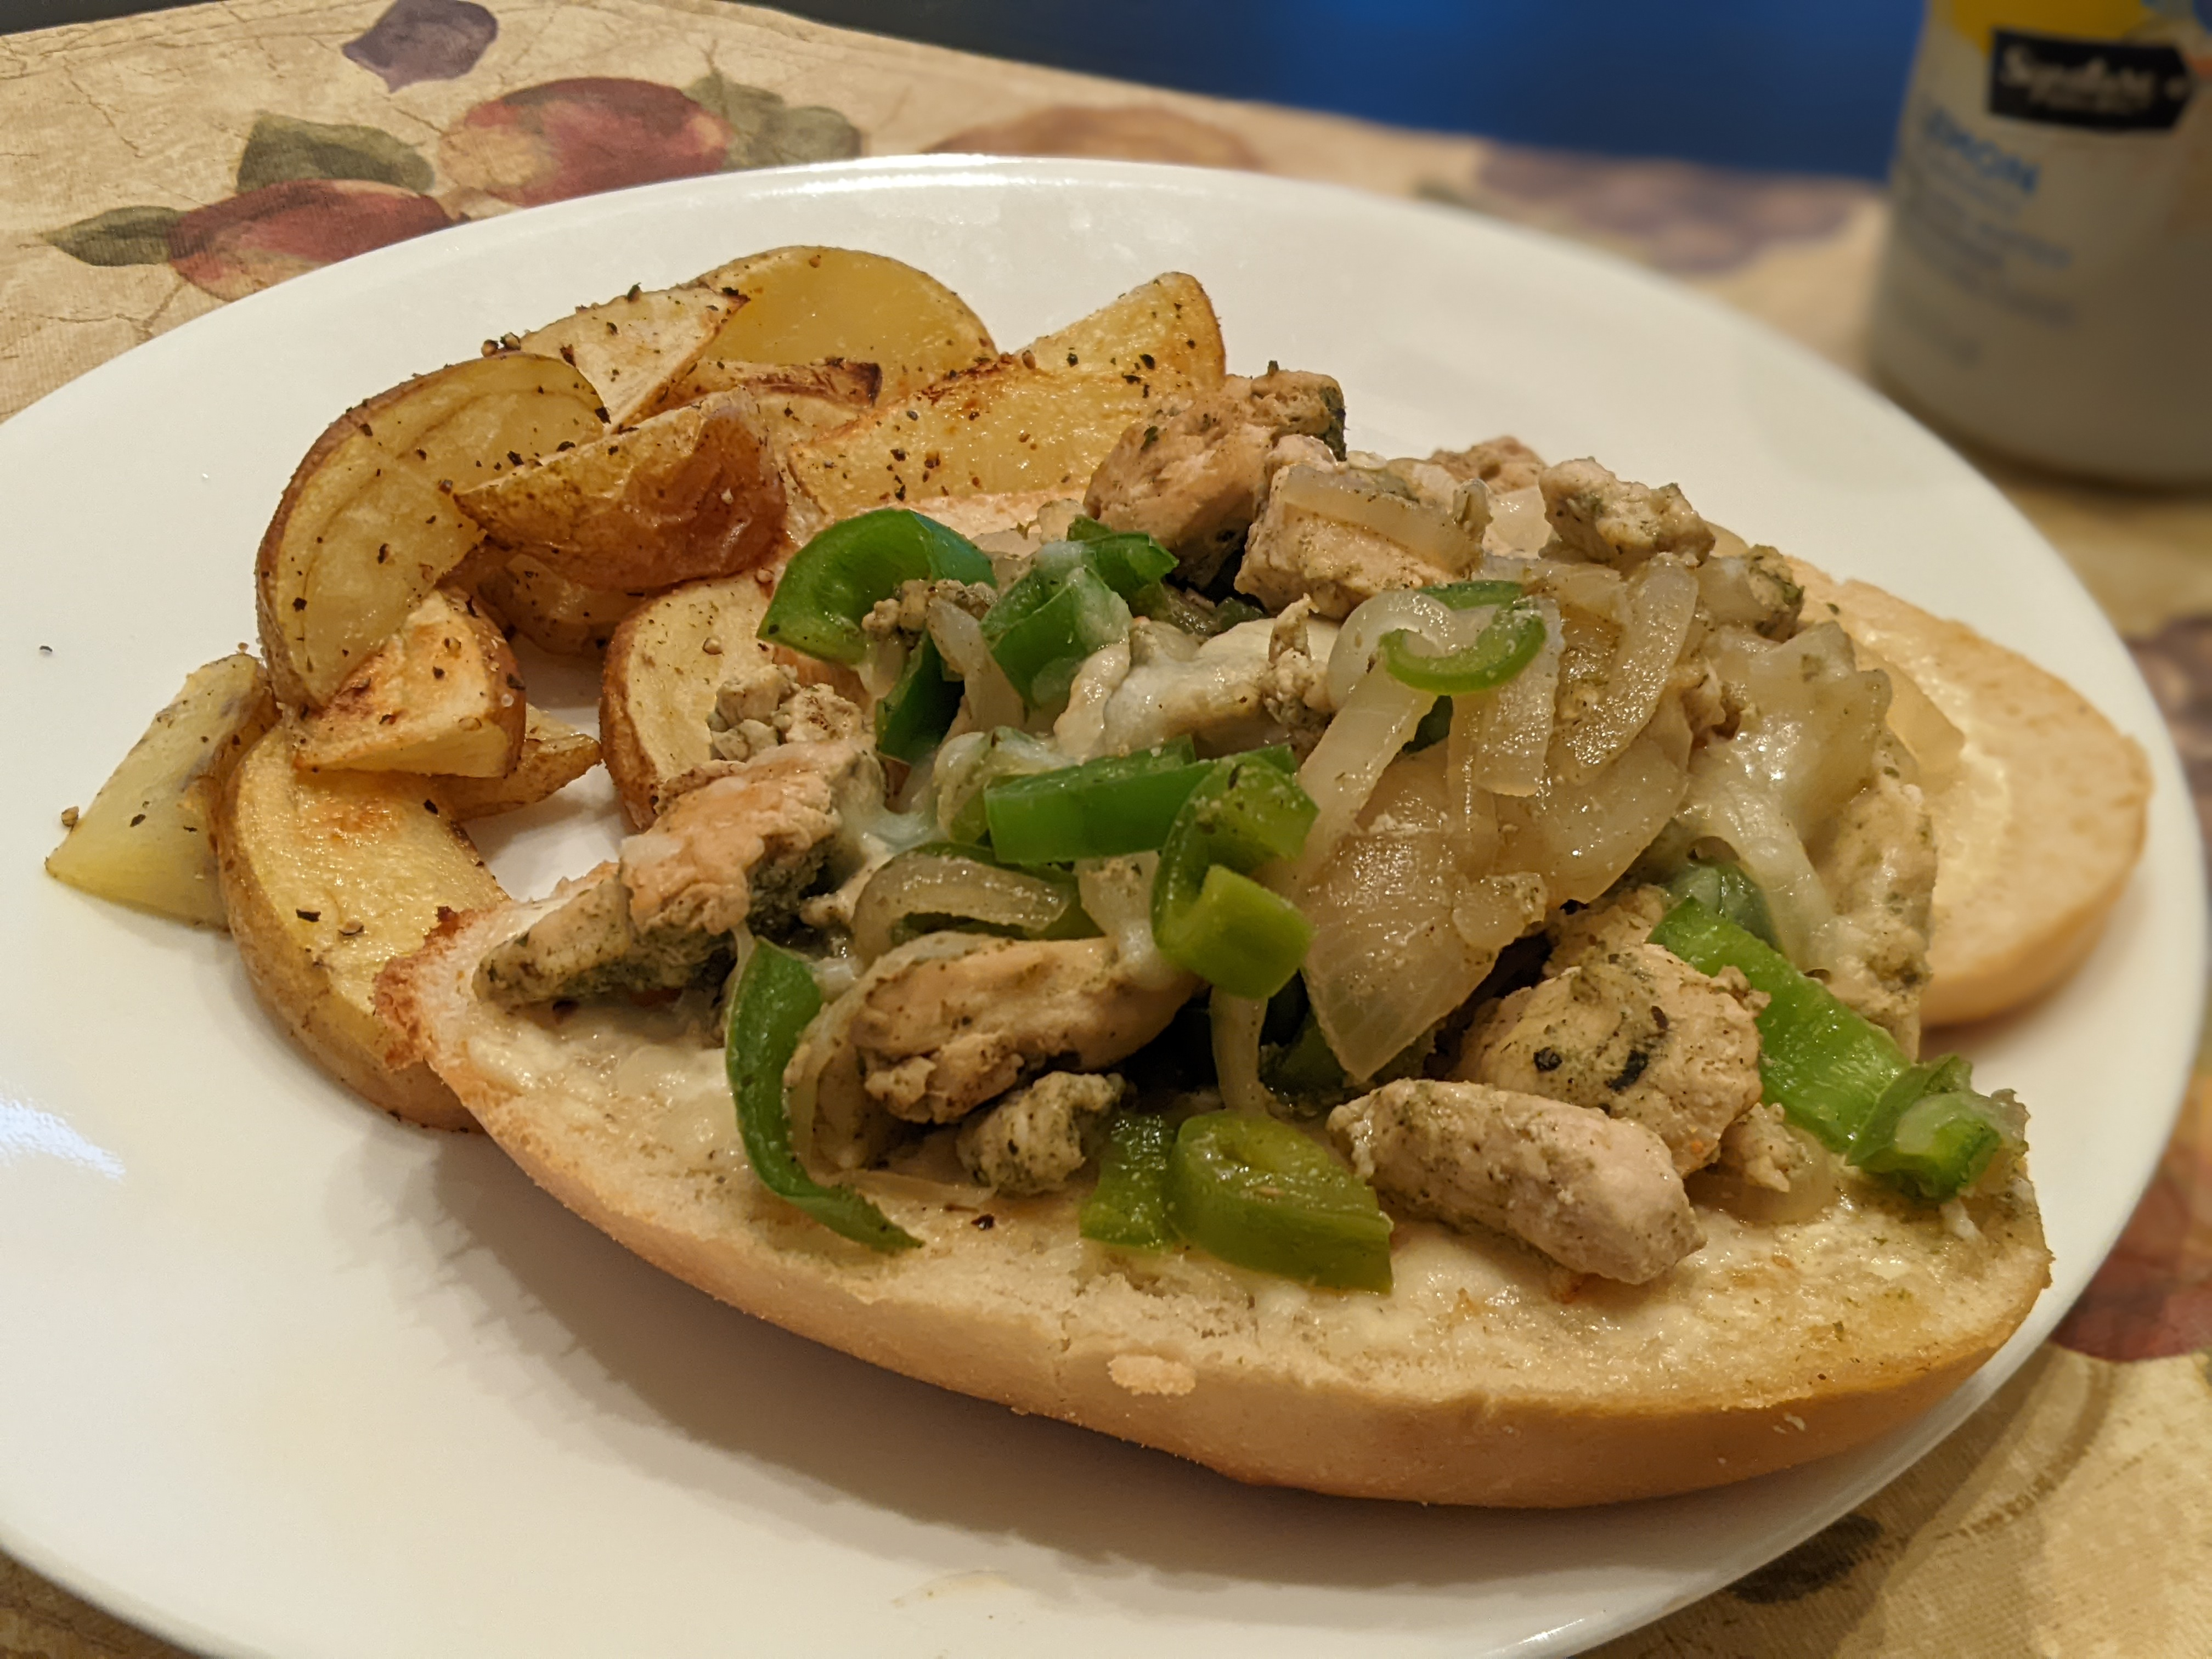
\includegraphics[width=5in]{photos/hello_fresh/italian_chicken_pepper_sandwich.jpg}
\end{center}